%%%%%%%%%%%%%%%%%%%%%%%%%%%%%%%%%%%%%%%%%%%%%%%%%%%%%%%%%%%%%%%%%%%%%%%%%%%%%%%
%%%%%%%%%%%%%%%%%%%%%%%%%%%%%%%%%%%%%%%%%%%%%%%%%%%%%%%%%%%%%%%%%%%%%%%%%%%%%%%
%%%%%%%%%%%%%%%%%%%%%%%%%%%%%%%%%%%%%%%%%%%%%%%%%%%%%%%%%%%%%%%%%%%%%%%%%%%%%%%

\section{Workflow zpracování textu}

V rámci nabízených možností je práce tématicky zaměřena především na
zpracování textu přirozeného jazyka (\textit{\underline{n}atural
\underline{l}anguage \underline{p}rocessing}, NLP) a dále na vývoj
vlastní aplikace, která poté se zpracovaným textem pracuje.

Nejdříve byly získány již existující korpusy anglických textů různého
původu (jde o texty pocházející z anglických zpravodajských relací, blogů
a z twitteru), jde o tzv. \textit{Helsinki corpora} [@Kytoo1996], které
jsou za určitých podmínek a pro určité účely dostupné online. K nim byl
přidán ještě menší korpus získaný vlastním webscrapingem malé části
anglicky mluvící Wikipedie. Korpusy byly poté jednotně předzpracovány.
Bloky textů korpusů byly nejdříve rozděleny na věty, a to podle určité
heuristiky. Dále byl text vět očištěn o některé nadbytečné znaky
(především interpunkci); v závěru této fáze jsou korpusy tvořeny
oddělenými větami, které tvoří písmena malé a velké anglické abecedy
a mezery. Velá písmena byla v rámci redukce "variability" textu převedena
bez ztráty infromace na malá písmena. Následovala fáze tokenizace vět
na jednotlivá slova, výsledkem tam byly pro každý korpus množina
uspořádaných, různě dlouhých $k$-tic slov, kde $k \geq 1$ je pro každou
větu nějaké přirozené číslo. V této fázi je možné odtsranit ta slova,
která v textech nejsou z nějakého smysluplného důvodu žádoucí. Jde
především o vulgarismy a jinak nevhodná slova (lze je očekávat hlavně
v korpusu pocházejícího ze sociální sítě \textsf{twitter}), dále je
možné (ale ne nutné) odstranit tzv. stop slova; jde obvykle o často
se objevující slova, většinou neohebných slovních druhů (není pravidlem),
která nenesou příliš zajímavou informaci.

Následně, když jsou korpusy zpracovány do té fáze, že jde o velké
množství uspořádaných $k$-tic vždy pro přirozená $k \geq 1$ lišící se
mezi původními větami, je možné text korpusů uchopit z pohledu
statistického modelování jazyka a nalézt v textu tzv. $n$-gramy pro malá
$n$, typicky $n \in \{2, 3, 4, 5\}$, ale i vyšší [@Manning1999].
Jde o $n$-členná sousloví, tedy $n$-tice sousedících, po sobě
jdoucích slov. Po sestavení $n$-gramů je možné vytvořit tabulku
četností pro jednotlivá $n$-členná slovní spojení a získat tak bodové
odhady apriorních pravděpodobností, s jakými se v textu daného
přirozeného jazyka vyskytují.

Takové tabulky četností $n$-gramů pro $n \in \{2, 3, 4, 5\}$ či vyšší
jsou základem pro algoritmy předpovědí takového slova, které by v textu
daného přirozeného jazyka následovalo s největší pravděpodobností po
zadaných $n - 1$ slovech. K tomuto účelu byla vytvořena webová aplikace
\texttt{the\_next\_word\_prediction}, která uživateli po zadání
$(n - 1)$-členného slovního spojení v daném jazyce vrátí
nejpravděpodobněji následující $n$-té slovo.

Angličtina je v rámci úlohy použita zcela záměrně -- jde o analytický
jazyk [@Gorblach1991], jehož textové a jazykově-statistické zpracování
je docela dobře možné, především díky minimálnímu zatížení anglických
textů morfematikou ohebných slovních druhů; lemmatizaci slov lze
v podstatě vynechat, aniž by byla ohrožena kvalita $n$-grammingu.
Opakem by byla čeština, tedy flekční jazyk, ve kterém je jazyková
analýza prakticky vždy závislá na kvalitě lemmatizace kvůli bohaté
morfologii s relativně vysokou mírou nepatternových vyjímek.


\subsection{Původ již existujících korpusů}

Jak již bylo naznačeno, největší část zpracovávaného textu pochází z tzv. \textit{Helsinki corpora}, což jsou rozsáhlé korpusy tematicky různorodých textů. Jsou za určitých podmínek a pro určité účely dostupné online, a sice na webu

\begin{center}
\href{http://www.helsinki.fi/varieng/CoRD/corpora/HelsinkiCorpus/}{\framebox{http://www.helsinki.fi/varieng/CoRD/corpora/HelsinkiCorpus/}.}
\end{center}

Volně stáhnout však korpusy nelze. Text, který však z korpusů vychází a je sestaven z těch částí helsinských korpusů, které jsou sesbírány z textů anglických\footnote{Vždy jde o americkou angličtinu, nikoliv britskou či jinou.} zpravodajských relací, anglicky psaných blogů a z anglicky psaných tweetů sociální sítě \textsf{twitter}, je možné získat v rámci absolvování masivního otevřeného online kurzu \href{https://www.coursera.org/specializations/jhu-data-science/}{\textit{Data Science}} na online univerzitě Coursera\textsuperscript{\textregistered}, který nabízí John Hopkins Bloomberg School of Public Health. Tato malá část původního korpusu je ke stažení např. zde

\begin{center}
\href{https://d396qusza40orc.cloudfront.net/dsscapstone/dataset/Coursera-SwiftKey.zip}{\framebox{https://d396qusza40orc.cloudfront.net/dsscapstone/dataset/Coursera-SwiftKey.zip}.}
\end{center}

Vzhledem k tomu, že kurz je volně dostupný a během něj je nakládání s odekzovanými částmi korpusů zcela v režii účastníka kurzu, zdá se, že nakládání s odkazovaným výňatkem korpusu není nelegitimní. Soubor v odkazu obsahuje i korpusy jiných jazyků než angličtiny.



\section{Metody zpracování textu}

V rámci relativně rozsáhlé fáze preprocessingu a processingu textových dat bylo nutné provést několik asynchronních úloh ("jednorázová předpočítání"), které byly náročné na vývojový i exekuční čas. Veškeré části úlohy byly naprogramovány a řešeny v prostředí \textsf{R}, které je určeno pro statistické výpočty a následné grafické náhledy [@Rlanguage]. Současně existuje online repozitář umístěný na platformě \textsf{GitHub} a obsahující všechny zdrojové kódy, kde je možné je i upravovat; je dostupný zde

\begin{center}
\href{https://github.com/LStepanek/4IZ470\_Dolovani\_znalosti\_z\_webu/tree/master/seminarni\_prace/}{\framebox{https://github.com/LStepanek/4IZ470\_Dolovani\_znalosti\_z\_webu/}.}
\end{center}


Veškerý komentovaný zdrojový kód je rovněž uveden ve stati "Implementace řešení asynchronních a synchronních úloh v \textsf{R}". I přes bohatou řadu knihoven pro \textit{text mining} a \textit{natural language processing}, kterou má jazyk \textsf{R} k dispozici, byly prakticky všechny funkce napsány "de novo" vlastními silami a jen s využitím základních klauzulí jazyka \textsf{R} (i ze cvičných důvodů); tedy bez použití dostupných intermediánních či vyšších vestavěných funkcí.

Schéma pořadí jednotlivých asynchronních úloh tak, jak byly v rámci zpracování textu prováděny, je naznačeno na obrázku \ref{pipeline_fig}.

\begin{figure}[H]
\centering
\begin{tikzpicture}[node distance=1cm, auto,]
  \node[punkt] (helsinki_corpora) {části helsinských korpusů};
  \node[punkt, right=1.0cm of helsinki_corpora] (webscraping) {webscrapovaný korpus z Wikipedie}
    edge[pil, bend left=45] (helsinki_corpora);
  \node[punkt, below=of helsinki_corpora] (sentence_splitting) {rozdělení všech korpusů na věty};
  \node[punkt, opacity=0, text opacity=0] (helsinki_corpora_dummy) {části helsinských korpusů}
    edge[pil, bend left=0] (sentence_splitting);
  \node[punkt, below=of sentence_splitting] (text_processing) {preprocessing textu};
  \node[punkt, below=of helsinki_corpora, opacity=0, text opacity=0] (sentence_splitting_dummy) {rozdělení všech korpusů na věty}
    edge[pil, bend left=0] (text_processing);
  \node[punkt, below=of text_processing] (tokenization) {tokenizace vět na slova};
  \node[punkt, below=of sentence_splitting, opacity=0, text opacity=0] (text_processing_dummy) {preprocessing textu}
    edge[pil, bend left=0] (tokenization);
  \node[punkt, below=of tokenization] (words_removing) {odstranění stop slov a vulgarismů, číslovek a krátkých slov};
  \node[punkt, below=of text_processing, opacity=0, text opacity=0] (tokenization_dummy) {tokenizace vět na slova}
    edge[pil, bend left=0] (words_removing);
  \node[punkt, below=of words_removing] (n_gramming) {$n$-gramming};
  \node[punkt, below=of tokenization, opacity=0, text opacity=0] (words_removing_dummy) {odstranění stop slov a vulgarismů, číslovek a krátkých slov}
    edge[pil, bend left=0] (n_gramming);
\end{tikzpicture}
\caption{Schéma (zjednodušené) asynchronních úloh během zpracovní textu pro účely $n$-grammingu \label{pipeline_fig}}
\end{figure}





\subsection{Webscraping Wikipedie}

Smyslem webscrapingu je stáhnout textový obsah nějakého počtu anglicky psaných stránek Wikipedie za účelem zvětšení celkového rozsahu všech použitých korpusů. Zároveň lze předpokládat, že vzhledem k tematickému zaměření části helsinských korpusů, kterou máme k dispozici, totiž texty zpravodajských relací (stručnější, gramaticky správné anglické fráze), blogů (jazykově bohaté, rozvité věty) a twitteru (krátká sdělení s velmi relaxovanou gramatikou), bude "korpus" získaný sloučením volných textů určitého množství stránek anglické Wikipedie nejen kvantitativním obohacením celkového užitého korpusu, ale do jisté míry i obohacením kvalitativním -- lze očekávat, že volný text ze stránek Wikipedie bude mít solidní gramatickou úroveň, půjde často o komplikovaná a dlouhá souvětí s hojným zastoupením idiomatických frází typických i pro akademickou anglickou mluvu.

Výhodou článků na Wikipedii je fakt, že jejich obsah (a v podstatě i většina formy) je uložen jen pomocí stacionárního HTML (\underline{H}yper\underline{T}ext \underline{M}arkup \underline{L}anguage). Formátování pomocí kaskádových stylů (CSS, \underline{C}ascading \underline{S}tyle \underline{S}heets), respektive aditivní javascriptovou funkcionalitu je sice na stránkách Wikipedie možné použít díky sdílení stylů a funkcí na Wikimedia Commons, běžné to rozhodně není; proto lze Wikipedii považovat za dobrý zdroj \textit{hard-typed} obsahu s pravidelnou (HTML) strukturou.

Pro účely webscrapingu jedné stránky Wikipedie byla napsána funkce

\begin{center}
\texttt{webscrapeMyWikipediaPage()},
\end{center}

jejímž vstupem je URL některé libovolné stránky typu článku anglické Wikipedie a výstupem je jeden textový řetězec, který je volným textem extrahovaným z textového obsahu stránky dané URL adresou. Funkce tedy desktopově stáhne veškerý HTML obsah dané URL adresy, poté extrahuje všechny řádky HTML kódu, které jsou ohraničeny HTML tagy \texttt{<p>} a \texttt{</p>}; ty totiž vymezují třídu HTML textu typu \texttt{paragraph} a víceméně jako jediné obsahují v rámci stránky volný text. Naopak ostatní HTML objekty typu nadpisy (vymezené tagy \texttt{<h$i$>} a \texttt{</h$i$>}), tabulky (vymezené tagy \texttt{<table>} a \texttt{</table>}) apod. bolný text neobsahují, resp. si tím nemůžeme být jistí, proto v rámci vysoké specificity scrapování pouze volného textu je obsah mezi tagy jinými než \texttt{<p>} a \texttt{</p>} ve výstupu vynechán.


Poté, co je extrahován volný text z HTML třídy \texttt{paragraph}, je ještě prosycen jinými HTML tagy (\texttt{<\ldots>\ldots</\ldots>}), HTML entitatmi (\texttt{\&\ldots;}) či wikipedickými tagy (obvykle \texttt{[\ldots]}). S aplikací Chomského hierarchie jazyků a Chomského pravidla [@Chomsky1956], že jazyk vyšší úrovně je třeba "značkovat" jazykem nižší úrovně (ve skutečnosti obecnějším, tedy metajazykem), byly už tak relativně obecné HTML klauzule z textu extrahovány pomocí regulárních výrazů. Snadno nahlédneme, že regulární výraz \texttt{<.*?>} odstraní všechny HTML tagy -- vyhledá totiž veškerý obsah (\texttt{.}) v libovolném množství (\texttt{*}) mezi úhlovými závorkami (\texttt{<\ldots>}), ale tak, aby např. v řádku \texttt{<p>Ahoj světe</p>} odstranil pouze HTML tag, nikoliv celý řádek; to vyjádříme otazníkem \texttt{?}, který regulárnímu výrazu říká "don't be greedy", tedy matchuje pouze nejkratší podřetězec daný regulárním výrazem. Obdobně regulární výraz \texttt{<\&.*?;>} matchuje "nehladově" všechny HTML entity a výraz \texttt{\textbackslash \textbackslash [.*? \textbackslash \textbackslash ]} naopak wikipedické tagy. Výsledkem takového očištění textových dat, původně charakteru HTML kódu, je pak volný text obsahující prakticky jen písmena abecedy, interpunkci a číslovky.

Kromě sestavení volného textu funkce z HTML obsahu extrahuje i všechny interní webové linky v rámci anglické Wikipedie; opět pomocí regulárního výrazu matchujícího pattern \texttt{href=''/wiki/\ldots''} typický pro wikipedický interní link.

Následovala procedura (ve skriptu \texttt{webscraping.R}), která na vstupu použila jeden zvolený článek, z něj vyextrahovala všechny interní outlinky vedoucí na jiné stránky typu článek anglické Wikipedie a současně scrapovala text tohoto článku. Outlinky byly uloženy do globální proměnné s linky. V druhé iteraci byla vyscrapována stránka (a do stejné globální proměnné s linky uloženy její outlinky) dostupná z prvního linku v globální proměnné s linky. V třetí iteraci byl proces opakován se stránkou odkazovanou druhým linkem v globální proměnné s linky. Proces byl opakován do chvíle, než bylo získo určité, uživatelem definované množství vyscrapovaných wikipedických stránek\footnote{Hypoteticky by mohla být procedura nechtěně ukončena i dříve -- a to např. tehdy, kdyby volba iniciální strány nebyla vhodná, protože by tato neobsahovala žádné outlinky, resp. by nějaké obsahovala, ale ty by vedly pouze na malé množství stránek, které by odkazovaly (jako izolovaný orientovaný graf) pouze samy na sebe (fenomén \textit{link farm sink}).}.

S volbou jednoho iniciálního anglicky psaného článku na Wikipedii, v našem případě konkrétně\footnote{Volba právě tohoto článku jako iniciálního nemá žádný hlubší smysl, ale článek obsahuje relativně velké množství volného textu.}

\begin{center}
\href{https://en.wikipedia.org/wiki/World\_War\_II}{\framebox{https://en.wikipedia.org/wiki/World\_War\_II}.}
\end{center}

a s podmínkou, že chceme vyscrapovat právě 900 wikipedických anglických stránek typu článek, byl nakonec sestaven vlastní (byť malý) "korpus" wikipedických stránek, uložený v souboru \texttt{en\_US.wikipedia.txt}. Jak bude dále naznačeno, dostupné části helsinského korpusu jsou samy o sobě natolik velké, že provedení asynchroních úloh nad textovými daty korpusu vyžaduje extermní množství výpočetního času.

Lze však dovodit, že uvedená webscrapovací funkce a procedura mohou v konečném čase teoreticky vytvořit rozsáhlý korpus ze stránek Wikipedie (budou-li tyto vzájemně dostatečně propojené interními linky), a to nejen anglické (algoritmus není citlivý na scrapovaný text).



\subsection{Dělení textu do vět}

Pro tuto úlohu byla implementována funkce 

\begin{center}
\texttt{splitTextIntoSentences()},
\end{center}

jejímž vstupem je textový řetězec celého odstavce a výstupem je určitý počet jednotlivých vět, na které je odstavec funkcí rozdělen. Algoritmu využívá regulárních výrazů, a sice je založen na pozorování, že na hranici dvou vět se vyskytuje prakticky vždy jeden z následujících patternů znaků:

\begin{itemize}
  \item sekvence tečka, mezera (žádá, jedna, nebo i více), velké písmeno -- tato sekvence je matchována regulárním výrazem \texttt{''\textbackslash \textbackslash .\textbackslash \textbackslash s*[A-Z]+''},
  \item sekvence otazník, mezera (žádá, jedna, nebo i více), velké písmeno -- tato sekvence je matchována regulárním výrazem \texttt{''\textbackslash \textbackslash ?\textbackslash \textbackslash s*[A-Z]+''},
  \item sekvence vykřičník, mezera (žádá, jedna, nebo i více), velké písmeno -- tato sekvence je matchována regulárním výrazem \texttt{''\textbackslash \textbackslash !\textbackslash \textbackslash s*[A-Z]+''},
  \item sekvence dvojtečka, mezera (žádá, jedna, nebo i více) -- tato sekvence odděluje nejspíše větu hlavní od věty vedlejší, což můžeme sémanticky vnímat jako dvě různé věty (alespoň pro účely $n$-grammingu); sekvence je matchována regulárním výrazem \texttt{''\textbackslash \textbackslash :\textbackslash \textbackslash s*''}.
\end{itemize}

Funkce relativně spolehlivě rozdělí libovolně dlouhý korpus o libovolném počtu vět na jednotlivé věty. Limitací funkce mohou být např. zkratky titulů, které budou matchovány první uvedenou sekvencí, ale ve skutečnosti nejsou na hranici dvou vět (v případě titulu \texttt{Ph.D.} je tento maskou pro pattern \texttt{''\textbackslash \textbackslash .\textbackslash \textbackslash s*[A-Z]+''}, dvě věty od sebe však jistě nerozděluje). Předpokládejme však, že půjde o relativně vzácný jev, který významně nenaruší další analýzu textu a $n$-gramming.

Dlužno říci, že jde o výpočetně náročnou úlohu: předpokládejme korpus délky $p$ symbolů, pak pro každou ze čtyř uvažovaných sekvencí mezi větami je tento korpus v lineárním čase proskenován (každá alespoň dvojice sousedních znaků je porovnána s regulárním výrazem), dostáváme tedy celkem $3(p-2)$ porovnání s patternem, pomocí asymptotické časové složitosti tedy $\Theta(3p) = \Theta(p)$. Pak, při průměrné délce $q$ symbolů jedné věty je předchozím porovnáváním nalezeno průměrně cca $\frac{p}{q}$ hranic sousedních vět, které jsou však sortovány jen v rámci sekvence. Je nutné tedy sortovat tři vektory o délce zhruba $\frac{p}{3q}$ rostoucích čísel dohromady, tím dostáváme výpočetní čas přinejmenším $\Theta(\frac{p}{q} \log \frac{p}{q})$ (merge sort). Nakonec je v lineárním čase $\Theta(\frac{p}{q})$ postupně ukrojena vždy "nová" první věta z postupně se zkracujího řetězce korpusu, jak "zpředu" vždy zkrácen o substring do prvního dalšího indexu označujícího novou hranici vět. Zřejme tedy rozdělení jednoho korpusu na věty běží v čase lehce náročnějším než lineárním, $\Theta(\frac{p}{q} \log \frac{p}{q})$, pro velká $p$ jde obecně o zdlouhavou proceduru.

Aktuálně je touto asynchronní úlohou zpracováno pouze cca 0,5 % dostupného korpusu -- není problémem rozdělit na věty celý korpus, avšak pro účely aplikace, která pak v daném seznamu $n$-gramů, jež roste s objemem vstupního korpusu, vyhledává vhodné zástupce $n$-gramů \textit{on-the-fly}, znamená příliš velký korpus velké zpomalení chodu aplikace.



\subsection{Preprocessing textu}

V rámci navazujícího preprocessingu textu jsou pomocí skriptu \texttt{preprocessing.R} provedeny v získaných větách tyto úpravy:

\begin{itemize}
  \item odstraněny zkratkové formy obsahující apostrof (např. \texttt{I'll} (I will)); jsou matchovány regulárním výrazem \texttt{''[a-zA-Z]+'[a-zA-Z]+''};
  \item odstraněny všechny znaky, které není možné kódovat pomocí UTF-8;
  \item všechna velká písmena jsou převedena na malá;
  \item všechny vícenásobné mezery jsou nahrazeny jednoduchou mezerou (\texttt{'' ''});
  \item odstraněny tzv. leading a trailing spaces (uvozující a koncové mezery); snadno nahlédneme, že ty nejsou předchozím krokem odstraněny;
  \item nakonec je z vět odstraněna veškerá intepunkce včetně závorek a dalších znaků netypických pro přirozený text (tedy hashtagů, zavináčů, smajlíkových forem apod.).
\end{itemize}



\subsection{Tokenizace}

Ve fázi, kdy je proveden kvalitní preprocessing a věty obsahují prakticky jen písmena malé anglické abecedy a jednoduché mezery, což vyplývá z operací provedených v rámci preporcessingu, je tokenizace vět na slova relativně snadnou úlohou. V rámci skriptu \texttt{tokenization.R} jsou namapovány indexy mezer ve větách a podle nich jsou pak věty rozděleny na slova pomocí uživatelem definované funkce \texttt{splitSentenceIntoWords()}. Výsledkem je tedy pro každý korpus tolik uspořádaných $k$-tic\footnote{$k$ zde není konstanta, variuje mezi jednotlivými větami.}, kolik obsahuje korpus vět; přirozené $k \geq 1$ udává pro každou větu počet slov, na které byla rozdělena.



\subsection{Odstranění stop slov a dalších}

Máme-li věty již rozděleny na slova, je možné některá slova odstranit, je-li k tomu speciální důvod. Na jedné straně je třeba si uvědomit, že odstraněním jednoho nebo více slov z věty, která je nyní reprezentována uspořádanou $k$-ticí, kde $k$ je počet jejích slov, můžeme narušit "sémantickou" plynulost věty, kterou je nepochybně vhodné udržet pro účely následného $n$-grammingu. V poslední době se objevují články, které odstranění stop slov, které bylo ještě donedávna pro některé typy především statistických úloh nad zpracováním přirozených textů rutinní fází, již nedoporučují, nebo ho minimálně zpochybňují, např. [@Saif2014]. Pravděpodobně to souvisí s rozvojem sofistikovanějších metod pro účely sémantické analýzy (např. sentiment analýzy), kde je vypuštění (stop) slov z vět vnímáno skutečně jako narušení jazykové kontinuity vět a jejich "přirozenosti", což nakonec zhoršuje výsledky sémantické analýzy. Navíc se běžně uváděné seznamy anglických stop slov významně liší. Z tohoto důvodu nebyla stop slova z vět v naší analýze odstraněna\footnote{Byť je pro to ve skriptu \texttt{postprocessing.R} vytvořena procedura.}. Progamrátorsky jde ale o relativně snadnou úlohu -- asymetrický rozdíl dvou uspořádaných seznamů zde vnímaných jako množiny, kdy od uspořádaného seznamu slov věty vnímaného jako množina (v Pythonu typicky \texttt{set(list)}) "odečítáme" množinu stop slov.

Naopak, odstraněna byla vulgární nebo jinak nevhodná slova, už jen z pragmatického důvodu určité serióznosti analýzy a na ní postavené aplikace. Nelze totiž vyloučit, že se nemohou nevohdná slova vyskytnout především v části korpusu pocházejícího ze sociální sítě \textsf{twitter}. Seznamů nevhodných slov (\textit{swear words lists}, \textit{profanity filters}) je online celá řada, např. \href{http://www.bannedwordlist.com/}{zde}.

Kromě nevhodných slov byly odstraněny ještě číslice, neboť jejich význam v dané větě je pouze kontextový; jsou-li součástí idiomatické fráze, u které máme zájem, aby byla součástí $n$-gramu, bude pravděpodobně vyjádřena číslovkou (slovem).



\subsection{$n$-gramming}

Vstupem pro $n$-gramming je uspořádaná $k$-tice slov, která reprezentuje $k$-slovnou větu. Korpus je pak složen z nějakého množství takto reprezentovaných vět. $n$-gramem rozumíme $n$-člennou sekvenci po sobě jsoucích slov některé $k$-slovné věty, přičemž předpokládáme, že $n \leq k$.

Snadno nahlédneme, že počet $n$-gramů, které můžeme získat z $k$-slovné věty, je roven $\epsilon(n, k)$ tak, že

\begin{equation*}
  \epsilon(n, k) = \left\{
  \begin{array}{rr}
  k - n + 1,  & n \leq k, \\
          0,  & n > k.
  \end{array} \right.
\end{equation*}

Algoritmus, který z korpusu získá všechny $n$-gramy, he relativně jednoduchý. V podstatě každou větu korpusu reprezentovanu uspořádaným seznamem slov proskenuje "čtecím okénkem" délky $n$ slov a vždy takový $n$-členné slovní spojení uloží do postupně rostoucího seznamu $n$-gramů.

Je-li v korpusu $l$ vět a je-li průměrná délka jedné věty $k$ slov, kde $k \geq n$, pak průměrná časová složitost algoritmu je asymptoticky $\Theta(l(k - n + 1)) = \Theta(kl-nl)$, tedy s rostoucím $n$ klesá.

Nad seznamem $n$-gramů lze vytvořit tabulka jejich frekvencí; relativní frekvence pak můžeme chápat jako bodové odhady pravděpodobností, s jakými se dané $n$-gramy vyskytují v textu příslušného přirozeného jazyka. Pro $n = 1$ získáme \textit{unigramy}, neboli jednotlivá slova. Pro $n = \{2, 3, 4, 5\}$ hovoříme postupně o \textit{bigramech}, \textit{trigramech}, \textit{quadriramech}, \textit{pentagramech}, respektive.

Seznamy $n$-gramů pro $\forall n = \{2, 3, 4, 5\}$ řeší implementovaná funkce \texttt{getNGrams()}, jejímž vstupem je jednak $n$, jednak věta reprezentovaná jako uspořádaná $k$-tice slov. Výstupem jsou všechny $n$-gramy, které lze z věty na vstupu získat. Skript \texttt{n\_gramming.R} počítá tabulky frekvencí pro jednotlivé $n$-gramy.



\section{Aplikace \texttt{the\_next\_word\_prediction}}

Aplikace, podobně jako asynchronní úlohy v rámci zpracování textu korpusů a $n$-grammingu, byla vyvinuta v jazyce \textsf{R} prostřednictvím \textsf{R}-kového balíčku \texttt{Shiny}.

Smyslem aplikace je nabídnout platformu pro predikci slova, které s největší pravděpodobností následuje zadané anglické $(n - 1)$-členné sousloví, $n > 1$.


\subsection{Princip aplikace}

Zadá-li uživatel do aplikace $(n - 1)$-členné anglické sousloví, kde $n > 1$, s cílem odhadnout slovo, které by mělo dané $(n - 1)$-členné sousloví s největší pravděpodobností následovat, aplikace najde největší takové $n_{0}$, aby $0 \leq n_{0} \leq n - 1$ a zároveň aby v množině všech $\{2, 3, 4, 5\}$-gramů existoval alespoň jeden takový $(n_{0} + 1)$-gram, že posledních $n_{0}$ slov uživatelem zadaného sousloví odpovídá postupně prvnímu, druhému, \ldots, $n_{0}$-tému slovu tohoto $(n_{0} + 1)$-gramu. Ze všech vyhovujících $(n_{0} + 1)$-gramů je pak vybrán ten, který má největší relativní četnost (v korpusu) a jeho $(n_{0} + 1)$-té slovo je vráceno uživateli jako to, které nejpravděpodobněji následuje jeho zadanou $(n - 1)$-člennou frázi.

Jinými slovy, uvažujme, že uživatel zadá do aplikace na vstupu $(n - 1)$-člennou frázi ve tvaru $w_{1}w_{2} \ldots w_{n - 1}$, kde $w_{j}$ je $j$-té slovo fráze pro všechna $j \in \{ 1, 2, \ldots, n - 1 \}$, s cílem zjistit, jaké slovo $w_{n}$ bude nejpravděpodobněji následovat po zadaných $n - 1$ slovech ve frázi. Buď $\mathcal{G}$ množina všech známých $n$-gramů pro všechna $n \in \{2, 3, 4, 5\}$. Hledáme $n_{0}$ takové, aby

\begin{equation*}
  n_{0} = \argmax_{i \in \{ 0, 1, \ldots, n - 1 \}} \{i : (\exists (i + 1)\text{-gram} = v_{1}v_{2} \ldots v_{i + 1} \in \mathcal{G})(\forall j \in \{1, 2, \ldots, i\})(v_{j} = w_{n - i + j - 1}) \}.
\end{equation*}

Je-li $n_{0} = 0$, aplikace vrátí nejčastější unigram (slovo \textit{the}). Je-li však $n_{0} > 0$, pak označme $\mathcal{G}_{w_{1}w_{2} \ldots w_{n - 1}}^{(n_{0} + 1)}$ množinu všech $(n_{0} + 1)$-gramů, které jsou tvaru $w_{n - n_{0}}w_{n - n_{0} + 1} \ldots w_{n - 1}$. Potom slovo, které nejpravděpodobněji následuje uživatelovu frázi $w_{1}w_{2} \ldots w_{n - 1}$, je $w_{n_{0} + 1}^{*}$ takové, že

\vspace{-1.5cm}
\begin{align*}
  \phantom{n_{0}} &\phantom{= \argmax_{i \in \{ 0, 1, \ldots, n - 1 \}} \{i : (\exists (i + 1)\text{-gram} = v_{1}v_{2} \ldots v_{i + 1} \in \mathcal{G})(\forall j \in \{1, 2, \ldots, i\})(v_{j} = w_{n - i + j - 1}) \}.} \\
  w_{n_{0} + 1}^{*} &= \argmax_{w_{n - n_{0}}w_{n - n_{0} + 1} \ldots w_{n - 1}w_{n_{0} + 1} \in \mathcal{G}_{w_{1}w_{2} \ldots w_{n - 1}}^{(n_{0} + 1)}} \{ \hat{P}(w_{1}w_{2} \ldots w_{n - 1}w_{n_{0} + 1} \mid w_{1}w_{2} \ldots w_{n - 1}) \}.
\end{align*}

Jde o MAP (\underline{m}aximum \underline{a}posteriori \underline{p}robability) princip, kdy je jako nejpravděpodobnější $n$-té slovo následující uživatelovu $(n - 1)$-člennou frázi vybráno poslední slovo takového $(n_{0} + 1)$-gramu, který má prvních $n_{0}$ slov totožných s posledními $n_{0}$ slovy uživatelovy fráze a zároveň je mezi takovými $(n_{0} + 1)$-gramy nejčastěji zastoupen. Je-li více takových nejčastěji zastoupených $(n_{0} + 1)$-gramů, je jako $n$-té slovo následující uživatelovu frázi vybráno to, které je první v abecedě. Někdy se též popsanému přístupu říká back-off model, neboť v podstatě nejdříve vyhledává shodu se zadanou frází mezi $5$-gramy (pentagamy); pokud ji nenajde, pokračuje mezi $4$-gramy (quadrigramy) atd. až k $1$-gramům (unigramům).



\subsection{Komponenty aplikace}

Aplikace se skládá z následujících částí:

\begin{itemize}
  \item \texttt{ui.R}
  \item \texttt{server.R}
  \item slovníky $n$-gramů, tedy \texttt{my\_$i$\_word\_vocabulary} pro $i \in \{1, 2, 3\}$
  \item složka \texttt{www}:
  \begin{itemize}
    \item \texttt{style.css}
  \end{itemize}
\end{itemize}


Uživatelský layout aplikace je relativně jednoduchý a intuitivní, viz obrázek \ref{layout_fig}. Online lze aplikaci používat snadno na adrese

\begin{center}
  \href{http://shiny.statest.cz:3838/the\_next\_word\_prediction/}{\framebox{http://shiny.statest.cz:3838/the\_next\_word\_prediction/}}.
\end{center}

Na první záložce \textit{Results} lze vložit vstupní frázi o délce 1-3 slov. Po kliknutí na tlačítko \textit{Predict the next word!} se v pravém panelu zobrazí slovo, které by mělo pravděpodobně jazykově následovat po vložené $(n - 1)$-členné frázi.

Na druhé záložce \textit{About} je zmíněno pár slov o účelu a principu aplikace.

\begin{figure}[H]
  \centering
  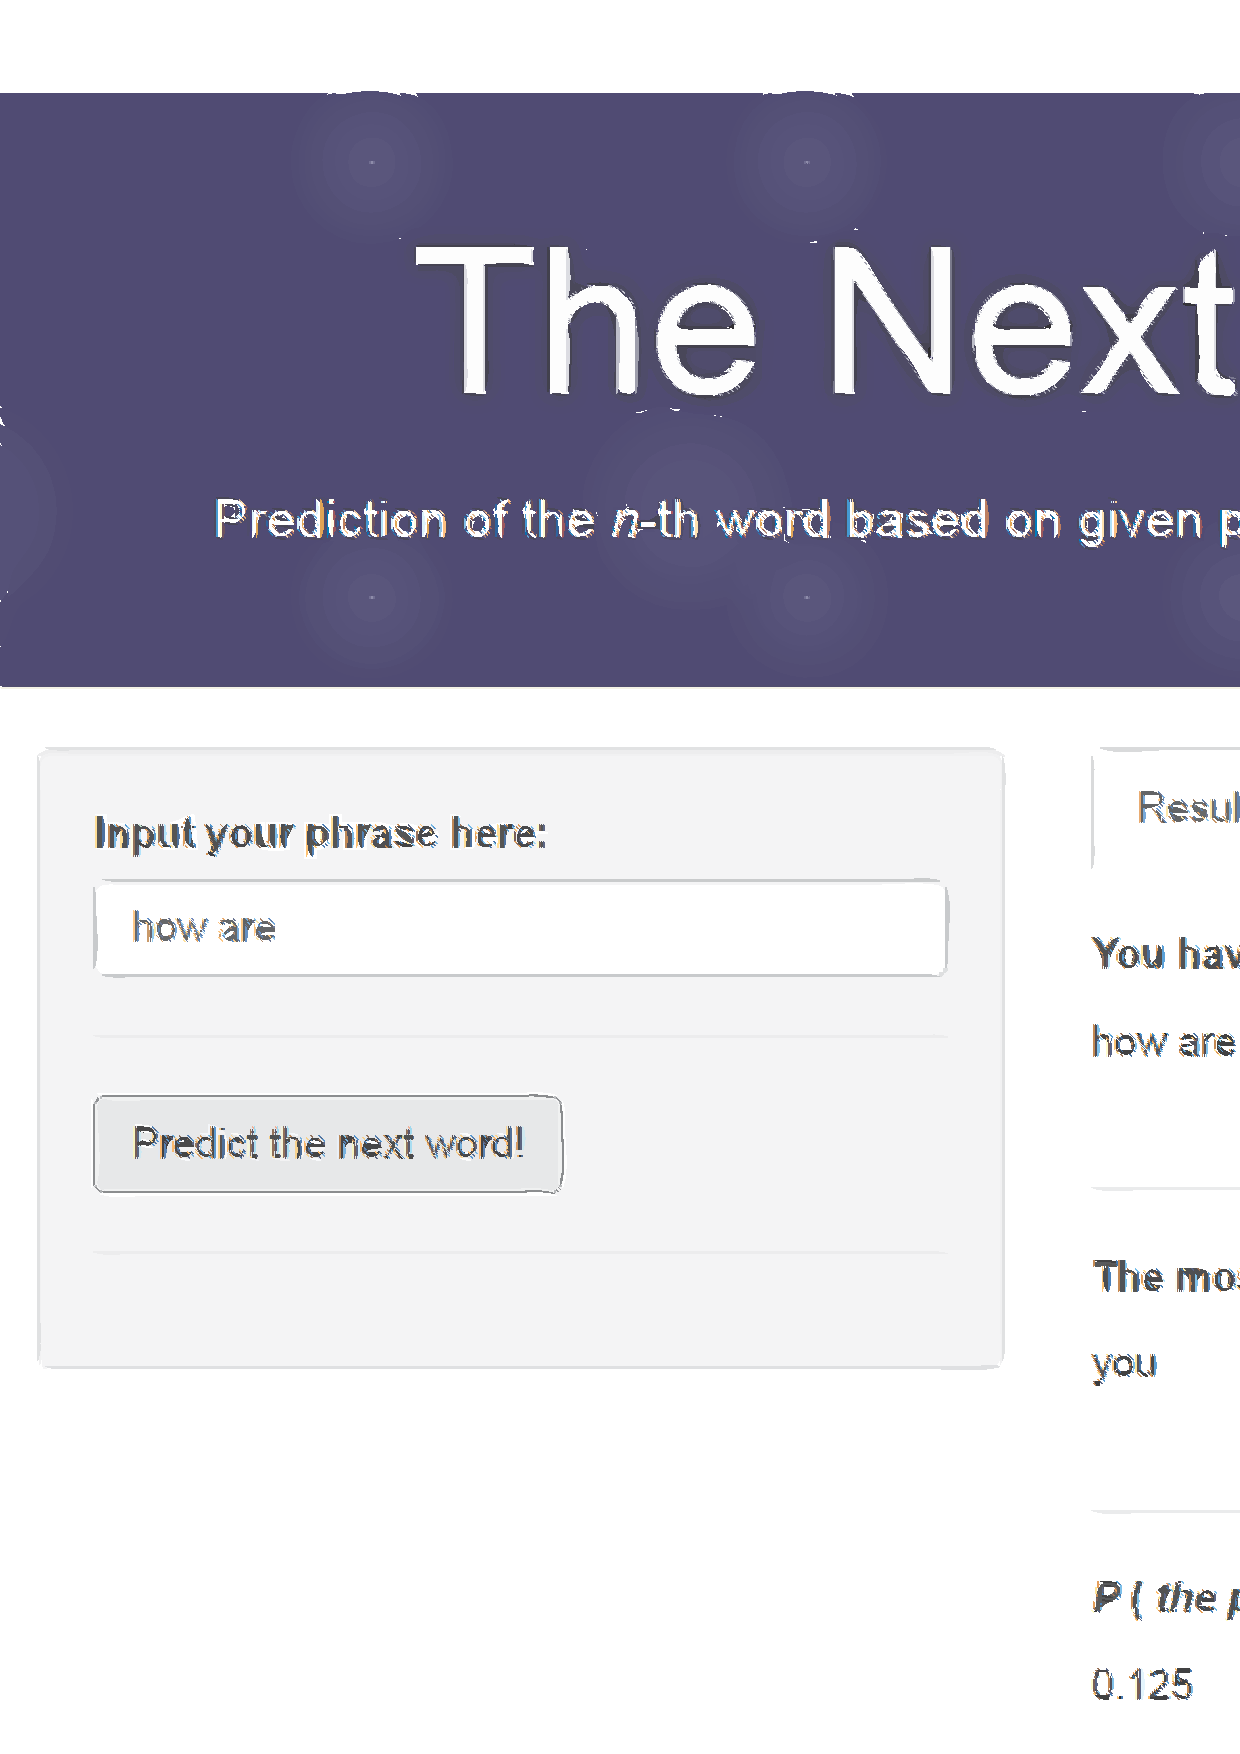
\includegraphics[height=12cm]{layout.jpg}
  \caption{Uživatelský interface domovské stránky aplikace}\label{layout_fig}
\end{figure}



Popišme nyní detailněji jednotlivé části aplikace.

\begin{labeling}{Conway\_Game\_of\_Life.myRscrip t}

  \item [\texttt{ui.R}] Název vyplývá z fráze \textit{\underline{u}ser \underline{i}nterface}. Definuje veškeré grafické a ovládací prvky aplikace, které lze napsat pomocí jazyka HTML (\underline{H}yper\underline{T}ext \underline{M}arkup \underline{L}anguage). I přesto je však psána pomocí příkazů jazyka \textsf{R}; balíček \textsf{Shiny} totiž definuje placeholderové funkce (aliasy), které mají na vstupu kód srozumitelný prostředí \textsf{R}, ale na výstupu vrací čisté HTML. Některé grafické prvky však byly napsány přímo pomocí syntaxe HTML -- balíček \textsf{Shiny} této syntaxi rozumí a v případě, že má uživatel znalost i značkovacího jazyka HTML, je pak práce snazší přímo pomocí HTML, nikoliv \textsf{R}-kových aliasů.
  
  \item [\texttt{server.R}] Jádro celé aplikace, obsahuje workhorse funkce, především implementaci backoff modelu výběru tak, jak je popsán ve stati "Princip aplikace".
 
  \item [\texttt{style.css}] Kaskádové styly, které definují rozměry, barvy a další parametry některých prvků aplikace, především headeru.

  
\end{labeling}




\section{Další možné směřování práce}

Nabízí se zpracování celého korpusu, eventuálně vytvoření $n$-gramů pro vyšší $n$. Zároveň je možné implementovat Kneser-Neyovo vyhlazování, které balancuje rozdíly mezi $n$-gramy a jejich kontextem pro malá a velká $n$. V aplikaci je možné nechat vypsat nikoliv jen první a nejpravděpodobnější slovo následující po zadané frázi, ale vypsat těchto slov hned několik a řadit je sestupně dle pravděpodobnosti.


\newpage


%%%%%%%%%%%%%%%%%%%%%%%%%%%%%%%%%%%%%%%%%%%%%%%%%%%%%%%%%%%%%%%%%%%%%%%%%%%%%%%
%%%%%%%%%%%%%%%%%%%%%%%%%%%%%%%%%%%%%%%%%%%%%%%%%%%%%%%%%%%%%%%%%%%%%%%%%%%%%%%
%%%%%%%%%%%%%%%%%%%%%%%%%%%%%%%%%%%%%%%%%%%%%%%%%%%%%%%%%%%%%%%%%%%%%%%%%%%%%%%





